% Syllabus Template from Arman Shokrollahi
% https://www.overleaf.com/latex/templates/syllabus-template-course-info/gbqbpcdgvxjs

\documentclass[11pt, letterpaper]{article}
%\usepackage{geometry}
\usepackage[inner=2cm,outer=2cm,top=2.5cm,bottom=2.5cm]{geometry}
\pagestyle{empty}
\usepackage{graphicx}
\usepackage{fancyhdr, lastpage, bbding, pmboxdraw}
\usepackage[usenames,dvipsnames]{color}
\definecolor{darkblue}{rgb}{0,0,.6}
\definecolor{darkred}{rgb}{.7,0,0}
\definecolor{darkgreen}{rgb}{0,.6,0}
\definecolor{red}{rgb}{.98,0,0}
\usepackage[colorlinks,pagebackref,pdfusetitle,urlcolor=darkblue,citecolor=darkblue,linkcolor=darkred,bookmarksnumbered,plainpages=false]{hyperref}
\renewcommand{\thefootnote}{\fnsymbol{footnote}}

\pagestyle{fancyplain}
\fancyhf{}
\lhead{ \fancyplain{}{Introduction to Political Methodology} }
%\chead{ \fancyplain{}{} }
\rhead{ \fancyplain{}{Fall 2020} }%\today
%\rfoot{\fancyplain{}{page \thepage\ of \pageref{LastPage}}}
\fancyfoot[RO, LE] {page \thepage\ of \pageref{LastPage} }
\thispagestyle{plain}

%%%%%%%%%%%% LISTING %%%
\usepackage{listings}
\usepackage{caption}
\DeclareCaptionFont{white}{\color{white}}
\DeclareCaptionFormat{listing}{\colorbox{gray}{\parbox{\textwidth}{#1#2#3}}}
\captionsetup[lstlisting]{format=listing,labelfont=white,textfont=white}
\usepackage{verbatim} % used to display code
\usepackage{fancyvrb}
\usepackage{acronym}
\usepackage{amsthm}
\VerbatimFootnotes % Required, otherwise verbatim does not work in footnotes!



\definecolor{OliveGreen}{cmyk}{0.64,0,0.95,0.40}
\definecolor{CadetBlue}{cmyk}{0.62,0.57,0.23,0}
\definecolor{lightlightgray}{gray}{0.93}



\lstset{
%language=bash,                          % Code langugage
basicstyle=\ttfamily,                   % Code font, Examples: \footnotesize, \ttfamily
keywordstyle=\color{OliveGreen},        % Keywords font ('*' = uppercase)
commentstyle=\color{gray},              % Comments font
numbers=left,                           % Line nums position
numberstyle=\tiny,                      % Line-numbers fonts
stepnumber=1,                           % Step between two line-numbers
numbersep=5pt,                          % How far are line-numbers from code
backgroundcolor=\color{lightlightgray}, % Choose background color
frame=none,                             % A frame around the code
tabsize=2,                              % Default tab size
captionpos=t,                           % Caption-position = bottom
breaklines=true,                        % Automatic line breaking?
breakatwhitespace=false,                % Automatic breaks only at whitespace?
showspaces=false,                       % Dont make spaces visible
showtabs=false,                         % Dont make tabls visible
columns=flexible,                       % Column format
morekeywords={__global__, __device__},  % CUDA specific keywords
}

%%%%%%%%%%%%%%%%%%%%%%%%%%%%%%%%%%%%
\begin{document}
\begin{center}
{\Large \textsc{POLS 7012: Introduction to Political Methodology}}
\end{center}
\begin{center}
{\large Fall 2020}
\end{center}

\begin{center}
\rule{6.5in}{0.4pt}
\begin{minipage}[t]{.96\textwidth}
\begin{tabular}{llcccll}
\textbf{Professor:} & Joe Ornstein & & &  & \textbf{Time:} & W 6:30 -- 9:15pm \\
\textbf{Email:} &  \href{mailto:jornstein@uga.edu}{jornstein@uga.edu} & & & & \textbf{Place:} & 102 Baldwin Hall\\
\textbf{Website:} & \href{https://uga.view.usg.edu/d2l/home/2058721}{https://uga.view.usg.edu/d2l/home/2058721} & & & & &
\end{tabular}
\end{minipage}
\rule{6.5in}{0.4pt}
\end{center}
\vspace{.15cm}
\setlength{\unitlength}{1in}
\renewcommand{\arraystretch}{2}

\begin{figure}[h]
	\centering
	\href{https://xkcd.com/1856/}{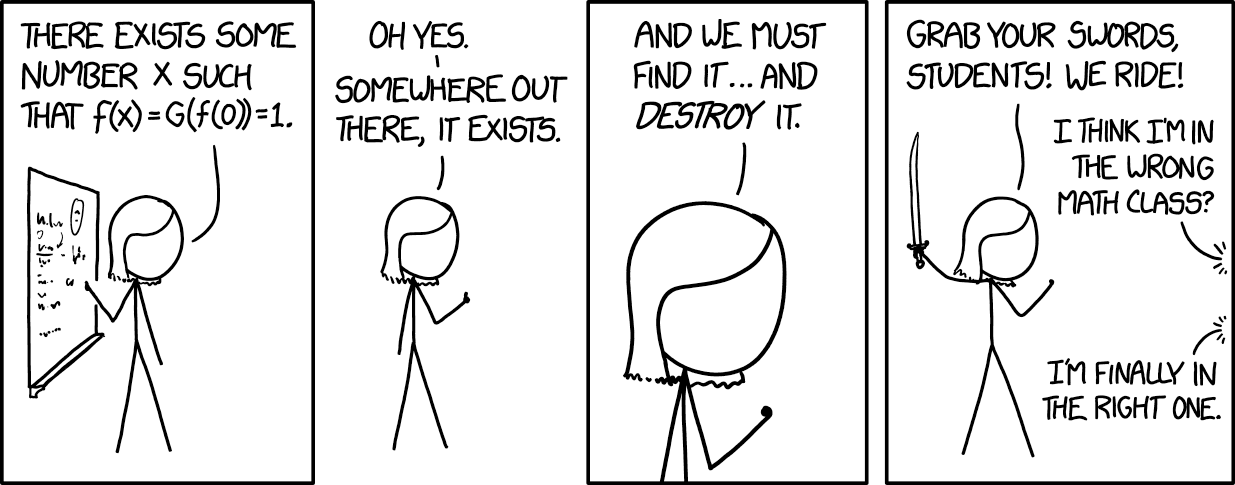
\includegraphics[width=0.8\textwidth]{img/existence_proof_2x.png}}
\end{figure}

%\begin{quotation}
%	\noindent``\textit{You can't really know anything if you just remember isolated facts. If the facts don't hang together on a latticework of theory, you don't have them in a usable form. You've got to have models in your head.}''\\
%	\\
%	--Charlie Munger (investor, vice chairman of Berkshire Hathaway)
%\end{quotation}

\noindent So you want to be a political scientist? Cool! It's a fun and fulfilling profession. But before you can eat your cake, you need to eat your vegetables. In this analogy, cake is political science, and vegetables is math. Because a lot of modern political science is heavily quantitative, and in order to fruitfully engage with the ongoing scientific conversation, you will need to understand the language. 

I intend for this class to be a very \textit{practical} introduction to the mathematical and computational skills you'll want to have as a professional political scientist. You'll learn how to manipulate, describe, and visualize data. You'll learn how to tell the difference between patterns in data and random noise. You'll learn how to fit models and make predictions. And when we're done, you'll have the fundamentals you need to tackle the advanced material that makes up the rest of the methods sequence. 

\section*{Course Objectives}
%\vskip.15in
%\noindent\textbf{Course Objectives:}  
By the end of this course, you will be able to:
\begin{itemize}
	\item Confidently work with data and create beautiful visualizations using the \texttt{R} programming language
	\item Organize your work so that it is transparent and reproducible
	\item Explain the fundamental mathematics behind the statistical methods we use in political science (probability and inference, matrix algebra, and optimization).
%	\item Manipulate, wrangle, and clean datasets using the \texttt{R} programming language
%	\item Create beautiful data visualizations
%	\item Organize your work so that it is transparent and reproducible
%	\item Compute derivatives and solve systems of linear equations
%	\item Explain the properties of probability distributions and expected values
%	\item Perform hypothesis tests and fit models to data
\end{itemize}

\section*{Course Structure}

This will be a weird semester, and I expect that there will be more than the usual share of setbacks and hardships. Please don't hesitate to ask questions or reach out to me with your concerns. 

If you show any \href{https://www.google.com/search?q=covid-19+symptoms}{symptoms of COVID-19} or have been exposed to someone who tests positive for COVID-19, don't come to class. Obviously. I do not grade class attendance, and every piece of material that you need to succeed on assignments and tests will be made available online. I plan to simulcast our class sessions over Zoom and post recordings to the course website, and I will hold regular virtual office hours if you have questions that aren't covered in those places. 

When you come to class, please wear a mask. The University System of Georgia (USG) requires all faculty, students, and staff to wear appropriate face coverings while inside campus buildings. Reasonable accommodations may be made for those who are unable to wear a face covering for documented health reasons. Students seeking an accommodation related to face coverings should contact Disability Services at \href{https://drc.uga.edu/}{https://drc.uga.edu/}. For more information on the University of Georgia's coronavirus response, visit \href{https://coronavirus.uga.edu/}{https://coronavirus.uga.edu/}. 

Our classroom will have a limited capacity this semester (14 students), but that should be sufficient to have all enrolled students attend in person. Following the Thanksgiving break, all remaining class sessions will be held online. 

\section*{Assignments \& Grading}

Each week, I will assign a problem set. Feel free to work with your classmates, but please submit your answers individually. 70\% of your grade will come from these problem sets, and 15\% each from a midterm and final exam. The midterm and final exam will both be online and open-book.

%\vskip.15in
%\noindent\textbf{Office Hours:} 
\section*{Office Hours}
Every Wednesday from noon to 1pm I will hold Virtual Office Hours over Zoom. I will put a sign-up spreadsheet on the course website. I'm also available before and after class to chat.

%\vskip.15in
%\noindent\textbf{Textbook:} %\footnotemark
\section*{Recommended Books}
I will not require you to purchase any books for this class, but here is a list of books you might find very useful:

\begin{itemize}
\item \href{https://r4ds.had.co.nz/}{Wickham, H., \& Grolemund, G. (2016). \textit{R For Data Science: import, tidy, transform, visualize, and model data}. O'Reilly Media, Inc.}

\item \href{https://www.amazon.com/All-Statistics-Statistical-Inference-Springer/dp/1441923225}{Wasserman, L. (2013). \textit{All of Statistics: A Concise Course in Statistical Inference}. Springer Science \& Business Media.}
\item \href{https://www.amazon.com/Mathematics-Economists-Carl-P-Simon/dp/0393957330}{Simon, C. P., \& Blume, L. (1994). \textit{Mathematics for Economists}. New York: Norton.}
\item \href{https://www.amazon.com/Visual-Display-Quantitative-Information/dp/1930824130}{Tufte, Edward (2001). \textit{The Visual Display of Quantitative Information}}
\item \href{https://socviz.co/}{Healy, Kieran (2018). \textit{Data Visualization: A Practical Introduction}. Princeton University Press.} 
\end{itemize} 



\section*{Tentative Course Outline}

Von Moltke writes that no battle plan survives first contact with the enemy. The same is true for syllabi. The following schedule is a rough outline that I may need to adjust on the fly. For instance, can I teach you everything you need to know about calculus in one week? Maybe! But if not, I've built in some Bonus Weeks towards the end of the semester that we can use for catch up. If everything goes according to plan, then we can cover extra topics during those weeks by popular demand.

%\begin{center} 
%\begin{minipage}{6in}
%\begin{flushleft}
%Chapter 1 \dotfill ~$\approx$ 3 days \\
%{\color{darkgreen}{\Rectangle}} ~A little of probability theory and graph theory	
\subsubsection*{Week 1: Getting Started}
\textit{Pre-Class Survey, Overcoming Fear, Notation, Setting up R and RStudio, Tidy Data, Basic Programming}

\subsubsection*{Week 2: Visualizing Data}
\textit{ggplot2, Tufte's Principles, Distributions, Correlations, Faceting}

\subsubsection*{Week 3: Tools for Reproducible Research}
\textit{Workflow, Documentation, File Structure, RMarkdown, \LaTeX, Zotero/Mendeley, \texttt{git} and GitHub}

\subsubsection*{Week 4: Tidying, Transforming, and Describing Data}
\textit{\texttt{tidyverse}, Merging, Filtering, Grouping}

\subsubsection*{Week 5: Functions}
\textit{Summation, Products, Logarithms, Exponentials, Writing Better Code, Flow Control}

\subsubsection*{Week 6: All The Calculus You Need}
\textit{Limits, Derivatives, Optimization, Integrals, Fundamental Theorem of Calculus}

\subsubsection*{Week 7: Probability}
\textit{Combinatorics, Random Variables, Expectation, Variance, Covariance, Conditional Probability, Bayes Rule, Law of Large Numbers}

\subsubsection*{Week 8: Inference}
\textit{PDFs and CDFs, Central Limit Theorem, Hypothesis Testing}

\subsubsection*{Week 9: Review \& Catchup}
\textit{Midterm Exam}

\subsubsection*{Week 10: Matrix Algebra and OLS}
\textit{Regression, Systems of Linear Equations, Independence, Matrix Multiplication, Matrix Inversion}

\subsubsection*{Week 11: Models and Prediction}
\textit{Fitting Models, Machine Learning, Overfitting, Cross-Validation, Regularization, Ensembles}

\subsubsection*{Week 12: Bonus Week 1}
Possible Topics: \textit{Causal Inference, Text-As-Data, Big Data, Machine Learning, Networks, Spatial Data, \texttt{blogdown, bookdown}, Advanced Reproducible Research}

\subsubsection*{Week 13: Bonus Week 2}
Possible Topics: \textit{Causal Inference, Text-As-Data, Big Data, Machine Learning, Networks, Spatial Data, \texttt{blogdown, bookdown}, Advanced Reproducible Research}

\subsubsection*{Week 14: Bonus Week 3}
Possible Topics: \textit{Causal Inference, Text-As-Data, Big Data, Machine Learning, Networks, Spatial Data, \texttt{blogdown, bookdown}, Advanced Reproducible Research}

\subsubsection*{Week 15: Review \& Catchup}
\textit{Final Exam}



%\end{flushleft}
%\end{minipage}
%\end{center}

%\vskip.15in
%\noindent\textbf{Important Dates:}
%\begin{center} \begin{minipage}{3.8in}
%\begin{flushleft}
%Midterm \#1      \dotfill ~\={A}b\={a}n 16, 1393  \\
%Midterm \#2      \dotfill ~\={A}zar 21, 1393  \\
%%Project Deadline \dotfill ~Month Day \\
%Final Exam       \dotfill ~Dey 18, 1393  \\
%\end{flushleft}
%\end{minipage}
%\end{center}



\subsection*{Academic Honesty}
Remember that when you joined the University of Georgia community, you agreed to abide by a code of conduct outlined in the academic honesty policy called \href{https://honesty.uga.edu/Academic-Honesty-Policy/Introduction/}{\textit{A Culture of Honesty}}. Problem sets may be completed in groups, but I expect your responses to be individual, and the midterm and final must be completed individually. 

\subsection*{Mental Health and Wellness Resources}

\begin{itemize}
\item If you or someone you know needs assistance, you are encouraged to contact Student Care and Outreach in the Division of Student Affairs at 706-542-7774 or visit \href{https://sco.uga.edu}{https://sco.uga.edu}. They will help you navigate any difficult circumstances you may be facing by connecting you with the appropriate resources or services. 
\item UGA has several resources for a student seeking \href{https://www.uhs.uga.edu/bewelluga/bewelluga}{mental health services} or \href{https://www.uhs.uga.edu/info/emergencies}{crisis support}. 
\item If you need help managing stress anxiety, relationships, etc., please visit \href{https://www.uhs.uga.edu/bewelluga/bewelluga}{BeWellUGA} for a list of FREE workshops, classes, mentoring, and health coaching led by licensed clinicians and health educators in the University Health Center.
\item Additional resources can be accessed through the UGA App.
\end{itemize}



%%%%%% THE END 
\end{document} 